% !TEX program = xelatex
\documentclass[10pt, aspectratio=169]{beamer}

\usetheme{metropolis}
\usefonttheme[onlymath]{serif}

\usepackage{fontspec}
\setsansfont{Hiragino Sans W3}[BoldFont={Hiragino Sans W6}]

\usepackage{amsmath, amssymb, amsfonts, mathtools}
\usepackage{tikz}
\usetikzlibrary{cd, arrows.meta, positioning, calc}
\tikzset{every node/.style={font=\sffamily}}
\usepackage{xcolor}

\definecolor{hilight}{HTML}{DBEAFE}
\definecolor{indigo}{HTML}{4338CA}
\definecolor{epsgreen}{HTML}{16A34A}
\definecolor{iotared}{HTML}{DC2626}

\newcommand{\hl}[1]{\colorbox{hilight}{\(\displaystyle #1\)}}

\title{最近 QFT (場の量子論) に少し入門したので話してみたい}
\author{@dokadokaas}
\date{}

\begin{document}

\maketitle

\begin{frame}{自己紹介}
  \begin{tikzpicture}[remember picture, overlay]
    \node[anchor=north east, inner sep=0pt] at ([xshift=-1cm, yshift=-1.5cm]current page.north east) {
      
\includegraphics[width=3.8cm]{assets/docker-whale.png}
    };
  \end{tikzpicture}
  \begin{itemize}
    \item \textbf{@dokadokaas}
    \item 興味は 数理物理 / 表現論 / 作用素環 / 確率論、最近は場の量子論を勉強中
    \item わかんなすぎること: 整数論 / 代数幾何
  \end{itemize}
\end{frame}

\begin{frame}{この発表の流れ}
\centering
\large
\textbf{$1+0$ 次元のクライン-ゴルドン場}

\medskip
{\color{gray}\small $\downarrow$ \quad 部分積分で落ちた境界項を拾う}

\medskip
\textbf{解空間 $\mathrm{Sol}$ とシンプレクティック形式}

\medskip
{\color{gray}\small $\downarrow$ \quad 正エネルギー部分から量子化}

\medskip
\textbf{場の量子論 $= (\mathcal{H}, \Phi)$}

\medskip
{\color{gray}\small $\downarrow$ \quad フォック空間 + 生成・消滅}

\medskip
\textbf{$\mathcal{H}$ と $\Phi$ の構成}
\end{frame}

\begin{frame}{$1+0$ 次元のクライン-ゴルドン場}
  \begin{columns}[T]
    \begin{column}{0.55\textwidth}
      \textbf{作用} $S$ は \textbf{場の集まり} $\mathcal{F}$ 上の関数
    \end{column}
    \begin{column}{0.4\textwidth}
      \begin{tikzpicture}
        \node[draw=blue!50, fill=blue!10, rounded corners, inner sep=5pt] (F) {$\mathcal{F}$ (場の集まり)};
        \node[right=1.2cm of F] (R) {$\mathbb{R}$};
        \draw[->, thick, indigo] (F) -- node[above] {$S$} (R);
      \end{tikzpicture}
    \end{column}
  \end{columns}

  \begin{center}\hl{S(\varphi) \coloneqq \int (|\dot{\varphi}|^2 - |\varphi|^2) \, dt \quad (\varphi: \mathbb{R} \to \mathbb{C})}\end{center}

  変分を取って \textbf{部分積分}  \begin{align*}
    \delta S &= \int \left[\dot{\varphi}\,\tfrac{d}{dt}\delta\bar{\varphi} + \bar{\dot{\varphi}}\,\tfrac{d}{dt}\delta\varphi - \varphi\delta\bar{\varphi} - \bar{\varphi}\delta\varphi\right] dt \\
    &= -\int \left[(\ddot{\varphi} + \varphi)\, \delta\bar{\varphi} + \overline{(\ddot{\varphi} + \varphi)}\, \delta\varphi \right] dt + \left[\dot{\varphi}\,\delta\bar{\varphi} + \bar{\dot{\varphi}}\,\delta\varphi\right]_{-\infty}^{\infty}
  \end{align*}

  境界項を捨てて、任意の $\delta\varphi$ で $\delta S = 0$ より \hl{\ddot{\varphi} + \varphi = 0} $\leftarrow$ \textbf{クライン-ゴルドン方程式}
\end{frame}

\begin{frame}{解空間とシンプレクティック形式}
  \textbf{解空間}  \begin{center}\hl{\mathrm{Sol} \coloneqq \{ \varphi \mid \ddot{\varphi} + \varphi = 0 \} = \{ pe^{it} + qe^{-it} \mid p, q \in \mathbb{C} \}}\end{center}

  部分積分で捨てた \textbf{境界項} を $\gamma$ にまとめ、$\mathrm{Sol}$ 上で \textbf{外微分} $\delta$ を取って $\omega$ を作る  \[ \gamma \coloneqq -\dot{\varphi}\delta\bar{\varphi} - \bar{\dot{\varphi}}\delta\varphi, \quad \omega \coloneqq \delta\gamma \]

  $\varphi = pe^{it} + qe^{-it}$ を代入して計算（略）すると、
  \begin{center}\hl{\omega_\mathrm{Sol} \coloneqq -2i(dp \wedge d\bar{p} - dq \wedge d\bar{q})}\end{center}

  $\leftarrow$ $\mathrm{Sol}$ 上の \textbf{シンプレクティック形式}
\end{frame}

\begin{frame}{場の量子論 = ヒルベルト空間 + 場の演算子}
  場の量子論は次の \textbf{2 つの組} のこと  \begin{center}\hl{\text{QFT} = (\mathcal{H}, \Phi), \qquad \Phi: \mathbb{R} \to \mathrm{End}(\mathcal{H})}\end{center}

  \begin{center}
  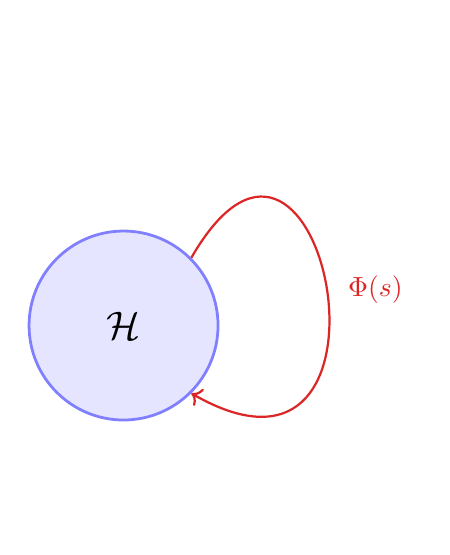
\begin{tikzpicture}
    \node[circle, draw=blue!50, fill=blue!10, line width=1pt, minimum size=2.4cm] (H) {\Large$\mathcal{H}$};
    \draw[->, thick, iotared] (H.45) to[out=60, in=-30, looseness=5] node[right=4pt, midway] {$\Phi(s)$} (H.-45);
  \end{tikzpicture}
  \end{center}

  \begin{center}\small 時刻 $s \in \mathbb{R}$ ごとに、$\mathcal{H}$ 上の演算子 $\Phi(s)$\end{center}
\end{frame}

\begin{frame}{$\mathcal{H}$ と $\Phi$ の構成}
\footnotesize
  \begin{columns}[T]
    \begin{column}{0.48\textwidth}
      \textbf{空間 $\mathcal{H}$}

      \smallskip
      $\mathrm{Sol}$ の \textbf{正エネルギー部分} $H_+ \coloneqq \{ pe^{it} \mid p \in \mathbb{C} \}$

      \smallskip
      \textbf{フォック空間} = \textbf{多項式環}      \begin{center}\hl{\mathcal{D} \coloneqq \bigoplus_n S^n H_+ = \mathbb{C}[e^{it}]}\end{center}

      内積 $(e^{ikt}, e^{ikt}) = k!$ で完備化して $\mathcal{H} \coloneqq \widehat{\mathcal{D}}$
    \end{column}
    \begin{column}{0.48\textwidth}
      \textbf{演算子 $\Phi$}

      \begin{center}\hl{\Phi(s) \coloneqq e^{is}\varepsilon + e^{-is}\iota}\end{center}

      \textbf{生成} $\varepsilon$：\hfill \hl{\varepsilon\, e^{ikt} \coloneqq e^{i(k+1)t} \ ({\color{epsgreen}\uparrow})}

      \smallskip
      \textbf{消滅} $\iota$：\hfill \hl{\iota\, e^{ikt} \coloneqq k\, e^{i(k-1)t} \ ({\color{iotared}\downarrow})}

      \begin{center}
      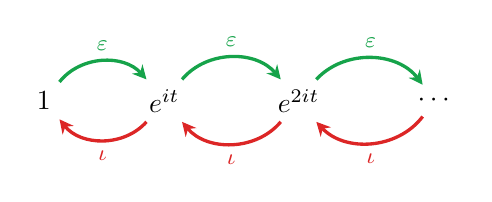
\begin{tikzpicture}[
        node distance=1cm,
        >={Stealth[length=5pt, width=5pt]},
      ]
        \node (n0) {$1$};
        \node[right=of n0] (n1) {$e^{it}$};
        \node[right=of n1] (n2) {$e^{2it}$};
        \node[right=of n2] (n3) {$\cdots$};
        \draw[->, color=epsgreen, line width=1.2pt] (n0) to[bend left=50] node[above, font=\footnotesize, color=epsgreen] {$\varepsilon$} (n1);
        \draw[->, color=iotared, line width=1.2pt] (n1) to[bend left=50] node[below, font=\footnotesize, color=iotared] {$\iota$} (n0);
        \draw[->, color=epsgreen, line width=1.2pt] (n1) to[bend left=50] node[above, font=\footnotesize, color=epsgreen] {$\varepsilon$} (n2);
        \draw[->, color=iotared, line width=1.2pt] (n2) to[bend left=50] node[below, font=\footnotesize, color=iotared] {$\iota$} (n1);
        \draw[->, color=epsgreen, line width=1.2pt] (n2) to[bend left=50] node[above, font=\footnotesize, color=epsgreen] {$\varepsilon$} (n3);
        \draw[->, color=iotared, line width=1.2pt] (n3) to[bend left=50] node[below, font=\footnotesize, color=iotared] {$\iota$} (n2);
      \end{tikzpicture}
      \end{center}
    \end{column}
  \end{columns}
\end{frame}

\begin{frame}{まとめ}
  ここまで作ってきた構成
  \begin{center}
  \begin{tikzpicture}[arrlbl/.style={font=\scriptsize, midway, above}]
    \node[fill=hilight, rounded corners, inner sep=5pt] (S) {$S$};
    \node[right=1.5cm of S, fill=hilight, rounded corners, inner sep=5pt] (EM) {運動方程式};
    \node[right=1.5cm of EM, fill=hilight, rounded corners, inner sep=5pt] (Sol) {$(\mathrm{Sol}, \omega_\mathrm{Sol})$};
    \node[right=1.5cm of Sol, fill=hilight, rounded corners, inner sep=5pt] (HPhi) {$\mathcal{H}, \Phi(s)$};
    \draw[->] (S) -- node[arrlbl] {$\delta S = 0$} (EM);
    \draw[->] (EM) -- node[arrlbl] {$\gamma, \omega$} (Sol);
    \draw[->] (Sol) -- node[arrlbl] {$H_+, \mathbb{C}[e^{it}]$} (HPhi);
  \end{tikzpicture}
  \end{center}

  でも、\textbf{時空に空間がない}（$1+0$ 次元）。$H \coloneqq \varepsilon\iota$ とおくと
  \begin{center}\hl{\Phi(s) = e^{isH}\Phi(0)\, e^{-isH}}\end{center}

  つまり $\Phi(s)$ は \textbf{位置演算子} $\Phi(0)$ の時間発展を書いてるだけ — \textbf{古典的な量子力学} の範疇でした

  \medskip
  \begin{center}
    \large でも、\textbf{空間ありでも同じ流れで構成できて、本当の場の量子論ができる}
  \end{center}
\end{frame}

\end{document}
